\documentclass{article}
\usepackage[utf8]{inputenc}
\usepackage{graphicx}
\graphicspath{ {./} }

\title{\textbf{Low-Poly Generator Project Proposal}}
\author{Rohan Jha - rjha@andrew.cmu.edu}
\date{November 16, 2019}

\begin{document}

\maketitle

\section{Project Description}
My 15-112 Term Project is called LowPolyGen. It generates a stylized, user-tuned, low-poly render of a given photo using Canny Edge Detection and Delaunay Triangulation algorithms. These generations will be displayed in an Adobe Bridge-style graphical recursive user file interface. In the interface, users will be able to interact with parameter sliders to re-render the low-poly image.

\section{Competetive Analysis}
First and foremost, I consider each of the following projects as inspiration, rather than competition; each takes the same base concept in different algorithmic and stylistic directions. I would identify Crystal Qian (cjqian on Github)'s polygen, Peter Maldonado (pmaldonado)'s PyTri, and Georg Fischer (snorpey)'s Triangulation webapp as the most comprehensive examples of competing projects. They span the gamut of delivery, purpose, and algorithmic approach from JavaScript web app to Python terminal call. Qian's implementation, as described in her paper (\textit{Generating low-poly abstractions}, Qian 2016)\footnote{http://cjqian.github.io/docs/tri\_iw\_paper.pdf} focuses primarily on subjective user opinion after an excellent mathematical portion detailing the effects of the well-chosen parameters of the algorithm (including sampling rate $\sigma$,  and blur) and, being more of an academic paper, has little emphasis on the surrounding infrastructure. On the other hand, Maldonado's implementation\footnote{https://github.com/pmaldonado/PyTri} has less focus, and is a more terminal-centric application, with many optional arguments that have less pertinence to the algorithmic side of the generation. Finally, Fischer's Triangulation web app\footnote{https://snorpey.github.io/triangulation/} demonstrates an appealing user experience, with near-real-time rendering on changed slider input, but this comes at the cost of a better refined product, specifically in how unintuitive the parameter's effects are on the output image.\\
In terms of dimensions of detail from other projects I'd like to pay close attention to in my own, Qian's thoughtful parameters merged with Fischer's sliders and image visualization rank very high. I do, however, forsee real-time generation based on user slider input as untenable due to the computational expense of my proposed algorithmic function. Instead, I will allow users to alter parameters with sliders, then lock them in and render with a button.


\section{Structural Plan}
LowPolyGen will be divided into four files, one handling preprocessing and the actual Delaunay generation of the images, one small one with a low poly image class, one handling the animation of the interactive Bridge-esque file system, and one wrapper file to ultimately run the experience.

\section{Timeline}
\begin{enumerate}
    \item TP1 (11/20)\\
    LowPolyGenerator image loading, preprocessing, edge detection, node threshold checking, and triangulation complete.
    \item TP2 (11/26)
    \begin{enumerate}
        \item By Friday Evening (11/22):\\
        Visual recursive file system animation, image compression (downsampling for time concerns), image thumbnail renders.
        \item By Saturday Night (11/23):\\
        Right side large display, parameter sliders that rerender image on button press.
        \item By Sunday Night (11/24):\\
        Testing and bugfixing.
        \item By Tuesday Meeting (11/26):\\
        Fully integrated file system with starting path select and slider/button rerenders.
    \end{enumerate}
    \item TP3 (12/5)
    \begin{enumerate}
        \item By Wednesday Night (11/27):\\
        Parameter translation functions to make sliders more user-intuitive.
        \item by Friday Night (11/29):\\
        Aesthetic refinements to Bridge interface. Continued generation optimization in hopes of real-time renders on slider change.
        \item by Sunday Night (12/1):\\
        Test and implement triangle area thresholding instead of vertex distance if not computationally prohibitive.
        \item by Tuesday Night (12/3):\\
        Final product done, rigorously tested.

    \end{enumerate}

\end{enumerate}

\section{Version Control}
For version control, I have initialized a private Github repository called Low-Poly-Generator. In addition to this, all supplemental materials like this proposal document, project notes, and image assets will be stored on Overleaf, Google Drive, and Imgur respectively.
\\
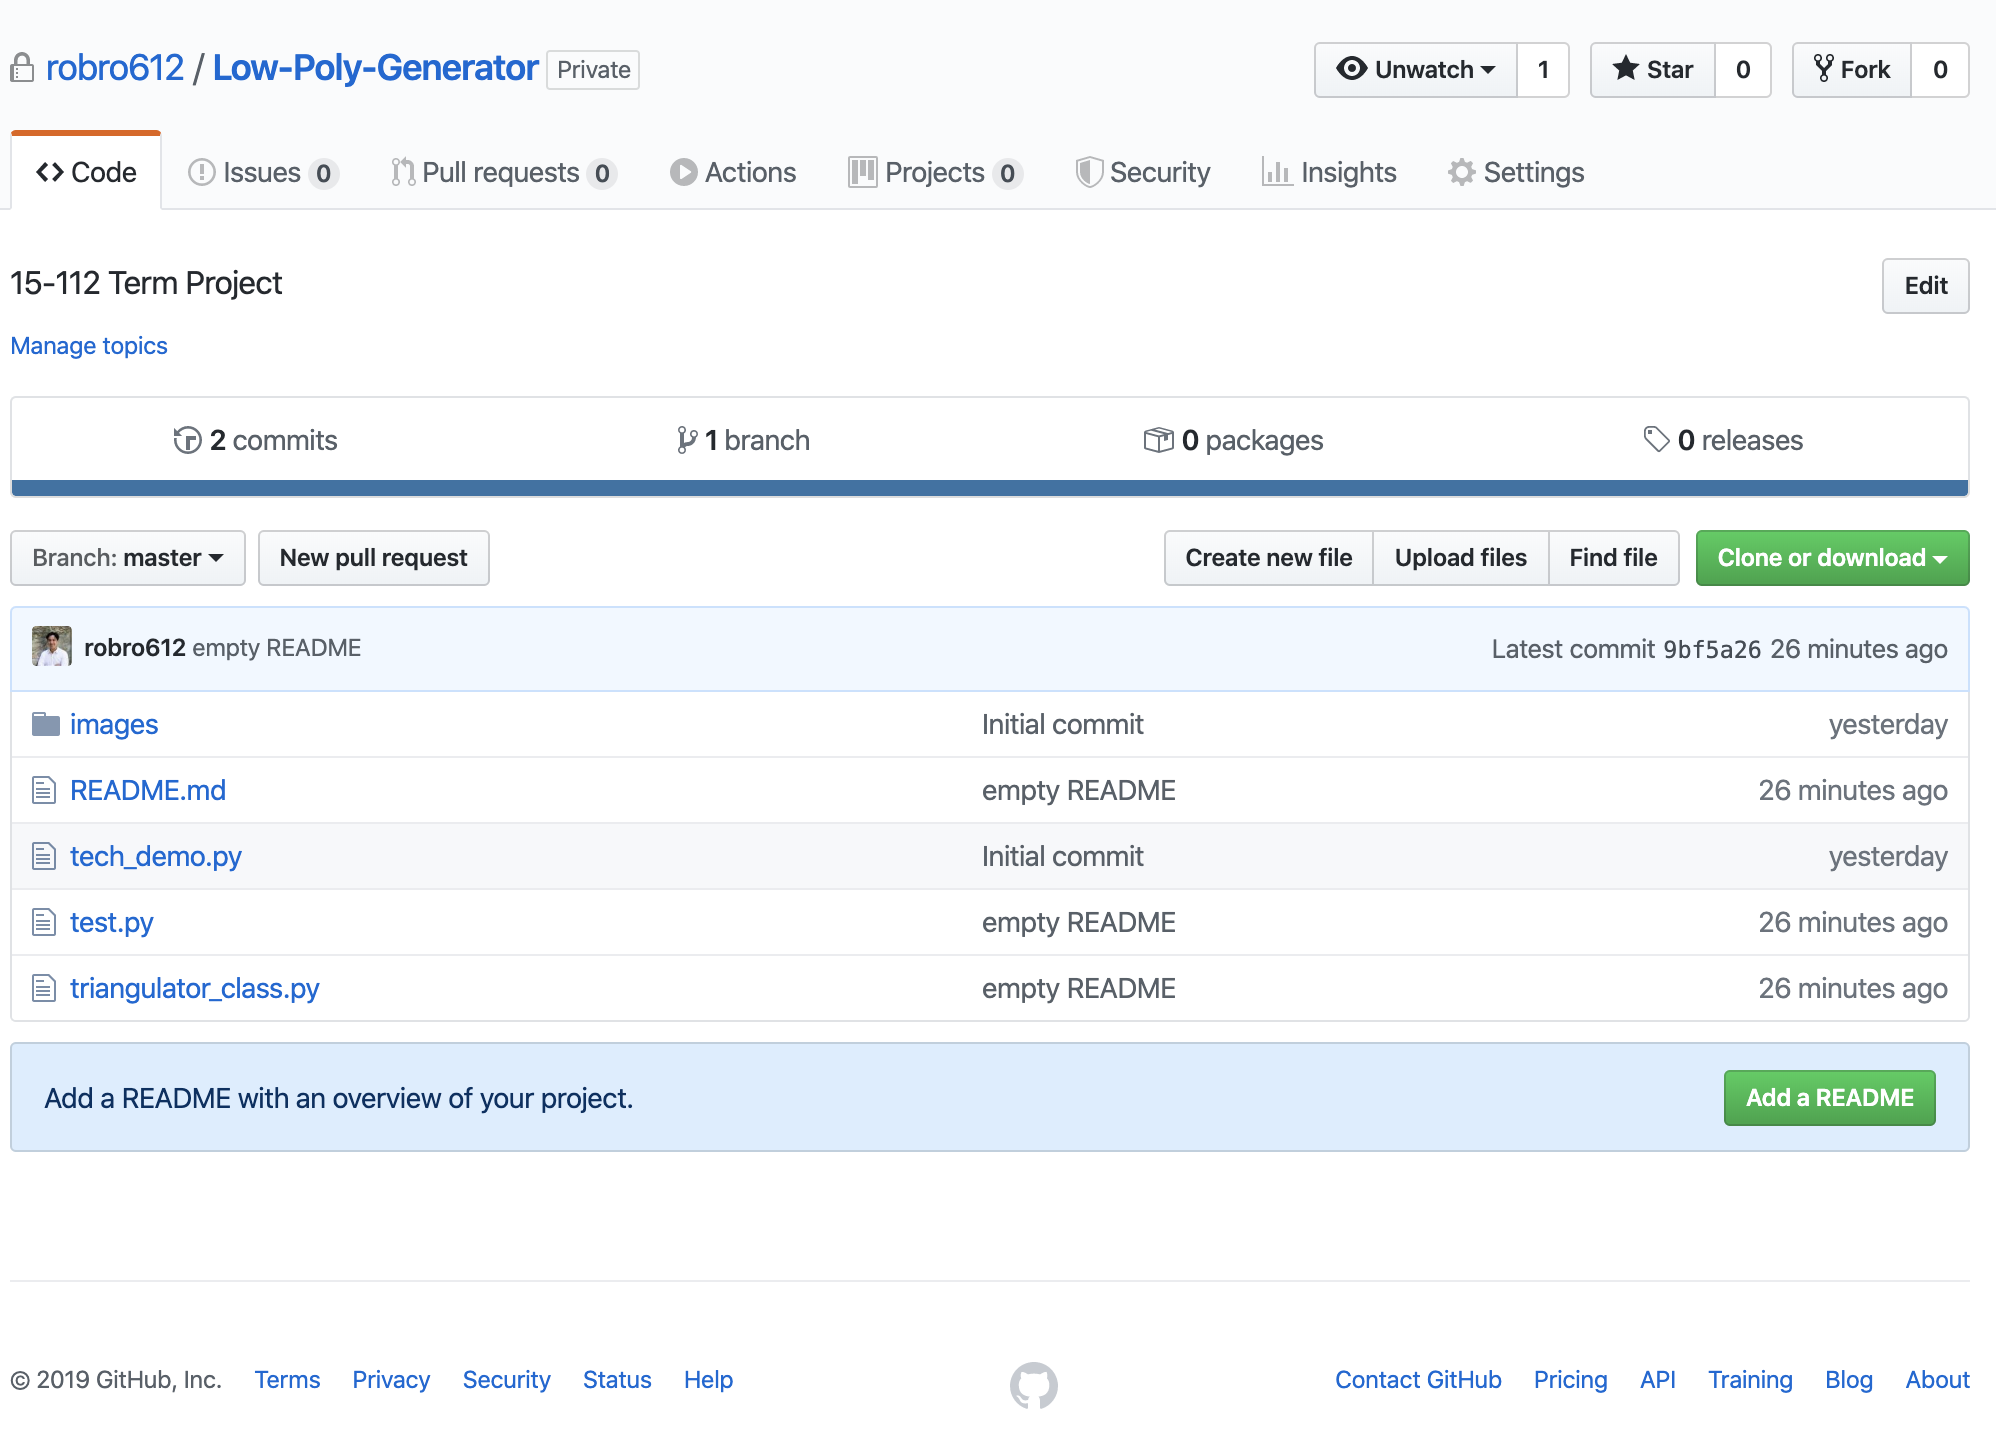
\includegraphics[scale = 0.3]{github.png}

\section{Module List}
I plan on using the following modules in my project:
\begin{enumerate}
    \item numpy for its highly optimized implementation of N-dimensional arrays in which we store our image pixel data as well as its seamless integration with matplotlib's plotting and cv2's convolutional filters.
    \item PIL for its baseline image crop and thumbnail functionalities.
    \item matplotlib for intermediate image and data visualization (currently blur, sharpen, and edge detection) as well as their slider implementation.
    \item cv2 for its convolutional filters, including blur, Canny edge detection, and a customizable filter with a user-set kernel.
    \item scipy for its implementation of Delaunay Triangulation, the algorithm that triangulates an image space $\Omega$ with triangles that have no other points in its circumcircle.
    \item tkinter and cmu\_112\_graphics for the final rendering and animation of the stylized image and surrounding user experience. Note that the graphics package is altered to not check for MVC violations in the draw function as it is critical to how I render the drawing without leaving the original window.
    \item random, time, and os for homemade Gaussian noise, efficiency testing, and file system interaction respectively.
\end{enumerate}

\section{Storyboard}
\centerline{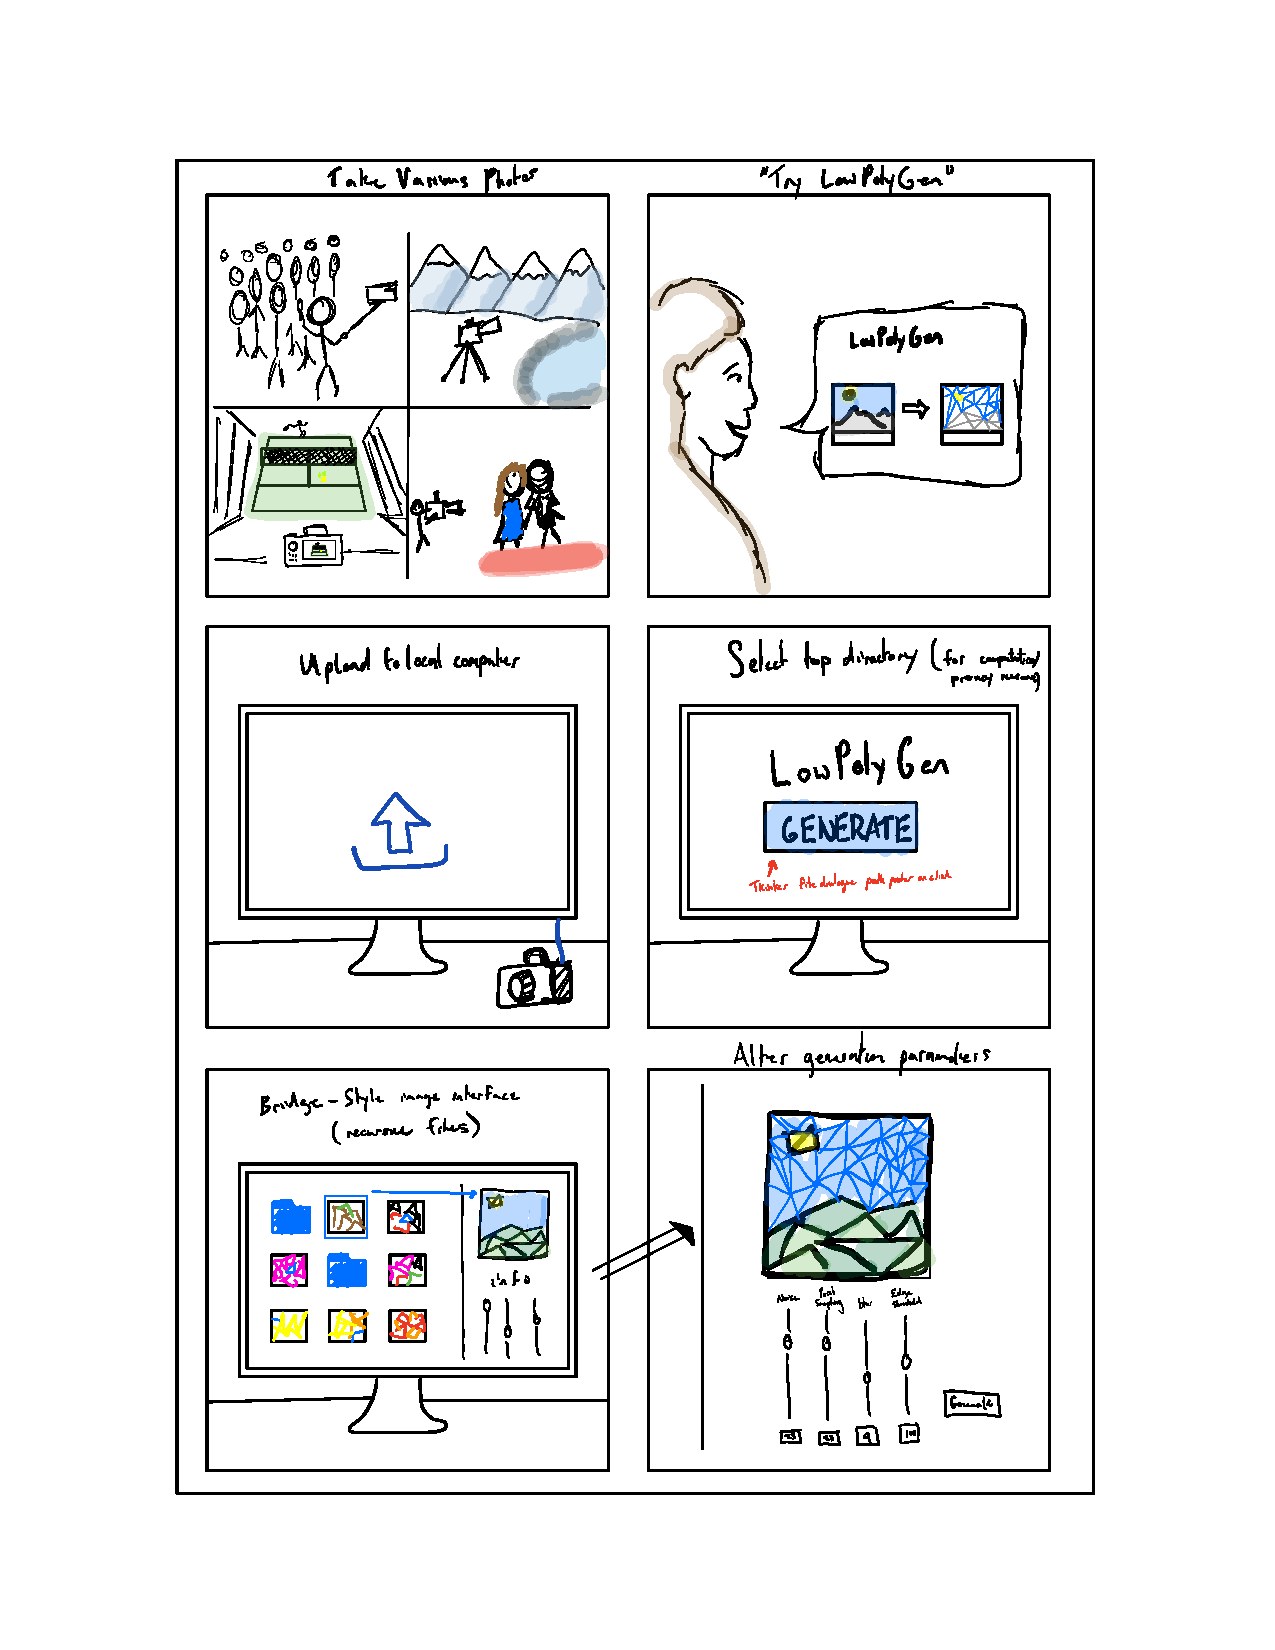
\includegraphics[scale = 0.8]{TP1.pdf}}
\end{document}
